\chapter{基于两方博弈的理性隐私风险访问控制模型}
\label{chap:game-theoretical-RaBAC-for-privacy}

\textit{本章。。。。}

\section{引言}

访问控制机制是解决信息和计算机社区中安全和隐私问题的基本技术。在当今的大规模,跨域和动态计算环境中,人们对隐私的关注日益增加,因此迫切需要灵活,细粒度,动态和自适应的访问模型。但是,传统的访问模型,例如自由访问控制(DAC)\cite{lampson1974protection},强制访问控制(MAC)\cite{bell1973secure}和基于角色的访问控制(RBAC)\cite{sandhu1996role}及其变体不能满足这样复杂而分散的计算环境和系统的要求。即使基于属性的访问控制(ABAC)\cite{kuhn2010}比传统的访问模型更灵活,更细粒度,并且更适合现代系统(例如ig云计算和大数据平台),仍然存在一些挑战\cite{servos2017,paci2018}。这些挑战源于日益增加的复杂性属性和用户,ABAC难以管理属性和策略,难以动态地监视和完善访问行为,因此仍然存在安全和隐私漏洞。

考虑卫生保健信息系统(HIS)的场景,一旦HIS识别出医生或护士,他(她)的访问策略将通过预定义的属性确定的和静态的,并且他(她)可以访问HIS中的所有敏感和私人医疗数据。根据他(她)的责任和义务,他(她)会访问过多的不必要的隐私数据,并且不会采取任何对策来监视和完善用户的访问权限。因此,侵犯患者隐私的行为时有发生。类似的情况也发生在机密信息系统,军事信息系统,社交网络等方面。为了缩小这一差距,克服传统访问模型(如dac、mac和rbac)和abac的不足,在访问控制中引入了风险\cite{cheng2007fuzzy, zhang2018privacy}和信任\cite{dimmock2004, pustchi2015},基于风险的访问控制(RBAC)\cite{cheng2007fuzzy}具有更强的隐私意识和适应性\cite{ni2010risk, wang2011quantified, zhang2018privacy}。


同时,访问主体始终与系统竞争并协作以访问对象。受试者希望从系统访问更多资源(包括正常所需的数据和额外的敏感数据)以获得有趣或商业上的利益。并且受试者必须与系统进行协作(尽可能遵循访问策略),以便他(她)可以获得更多访问机会。相反,系统希望识别所有异常和恶意访问,并且系统还希望与主题合作以吸引更多主题和访问请求。主体与系统之间的关系类似于博弈论\cite{nash1950},这是一种解决系统中理性参与者之间的冲突与合作的数学方法。博弈论在安全和隐私社区中发挥着重要作用\cite{do2017,zhu2018,tian2019}。而且,通过结合不同的功能,将博弈论借用到访问控制机制的设计中。\cite{hu2014,zhang2015,liu2016,gao2018, helil2017}。在以前的工作中,它适用于有限场景\cite{hu2014,gao2018}或辅助信息过多的场景\cite{zhang2015,liu2016,helil2017}。此外,将博弈论与访问控制结合起来的工作几乎都集中在安全性问题上(例如\cite{helil2017}是用于同时具有信任和风险评估的安全性)而不是隐私,因此访问之间仍然存在组合的潜在空间控制和博弈论,特别是用于数据和用户集中环境中的隐私保护。

旨在弥补访问控制模型中授权用户的隐私泄露漏洞,并克服先前工作的不足。在本文中,我们将信息熵和博弈论应用于基于风险的访问控制中,并设计了基于风险适应性的访问控制模型,用于私有数据和用户集中信息系统中的隐私保护。在提出的访问模型中,利用shannon信息、框架和工作流设计了访问请求和用户的风险值。通过引入新的组件,提出了基于风险的访问控制理论,并对基于风险的访问控制博弈模型进行了分析。通过实现纳什均衡,通过限制侵犯隐私的访问请求,有效地保护了隐私敏感资源。与之前的工作相比,这种方法可以使更多的特性受益。


与现有工作相比,我们的贡献如下。
\begin{itemize}
	
	\item 我们通过使用目标资源和访问资源的距离定义了新的概念:\textit{隐私风险}和\textit{隐私侵犯访问}。
	\item 我们提出了一个基于风险自适应的访问控制(RaBAC)的博弈论框架,并给出了基于xacml的访问控制流程。
	该框架涉及用户上下文,资源上下文,访问历史记录,风险历史记录和博弈历史记录。
	\item 我们使用信息度量和自定义功能来评估访问请求和用户的风险值。
	\item 我们分析服务提供商和用户之间的多阶段博弈,并获得每个阶段的纳什均衡,在这种状态下,可以有效地限制对隐私权的访问。
\end{itemize}


本章的其余部分,在\ref{sec:preliminaries}中简要介绍了一些基本知识之后,在\ref{sec:notations}中介绍了新提案的一些符号和模型,然后提出了具有演化博弈论的风险自适应访问控制模型, 在\ref{sec:framework}部分。 然后,在\ref{sec:riskvalue}部分介绍了风险评估方法,并在\ref{sec:gamemodel}部分介绍了有关访问模型的博弈分析。 在 \ref{sec:conclusions}部分,我们模拟了模型并获得了一些不错的结果。
最后,我们在本节中完成工作

\section{基于风险的访问控制模型}
\label{sec:preliminaries}

Cheng等\cite{cheng2007fuzzy} 介绍了第一种用于多级证券的风险量化方法访问控制模型,Ni等人\cite{ni2010risk} 通过将访问风险估计和模糊推理用于基于风险的访问控制,开发了工作\cite{cheng2007fuzzy}。使用符号\emph{risk}表示访问控制决策过程。与其他访问模型不同,我们还引入了\emph{operational need} 和\emph{situational factors}的概念来评估访问风险。 在大多数文献\cite{cheng2007fuzzy,ni2010risk,kandala2011,bijon2012}中,风险由函数 $f(\cdot, \cdot)$定义。在主体 $s$和对象$o$之间。 Cheng el等人\cite{cheng2007fuzzy}使用了主题之间的“差距”和对象的安全级别,即$risk(s,o)=Val(o) \cdot P(s,o)$,其中$Val(o)$是披露对象时损害的价值估算值, $P(s,o)$ 是披露的可能性。 此外,所有风险的定量定义都是相同的,类似于\cite{cheng2007fuzzy}的公式。 风险估计的数学公式为
\begin{equation}\label{eq:naive_risk}
Risk = Likehood \cdot Impact
\end{equation}

其中$Risk$是有关基本访问请求的定量值,$Likehood$ 表示事件发生的可能性,$Impact$ 表示事件的潜在损害的值。


在基于风险的访问控制模型中,总是有三个常见的组件,包括访问控制管理器,风险估计和上下文检索。在图\ref{fig:rbac}中,给出了从 \cite{diep2007}借用的基于风险的访问控制的概述。访问控制管理器组件接收访问请求,收集并分析用户的访问信息,然后将这些信息发送到风险估计组件。上下文检索组件收集上下文信息并发送给风险估计组件;风险估计组件通过使用从访问控制管理器和上下文检索组件收集的数据来评估每个访问请求的风险值,然后将风险值返回给访问控制管理器进行决策。基于风险的访问控制模型的核心问题是如何设计一种细粒度且适应性强的风险估计方法,而一种可适应的风险估计基础访问控制称为基于风险适应性的访问控制(RaBAC)。
\begin{figure}[htb]
	\centering
	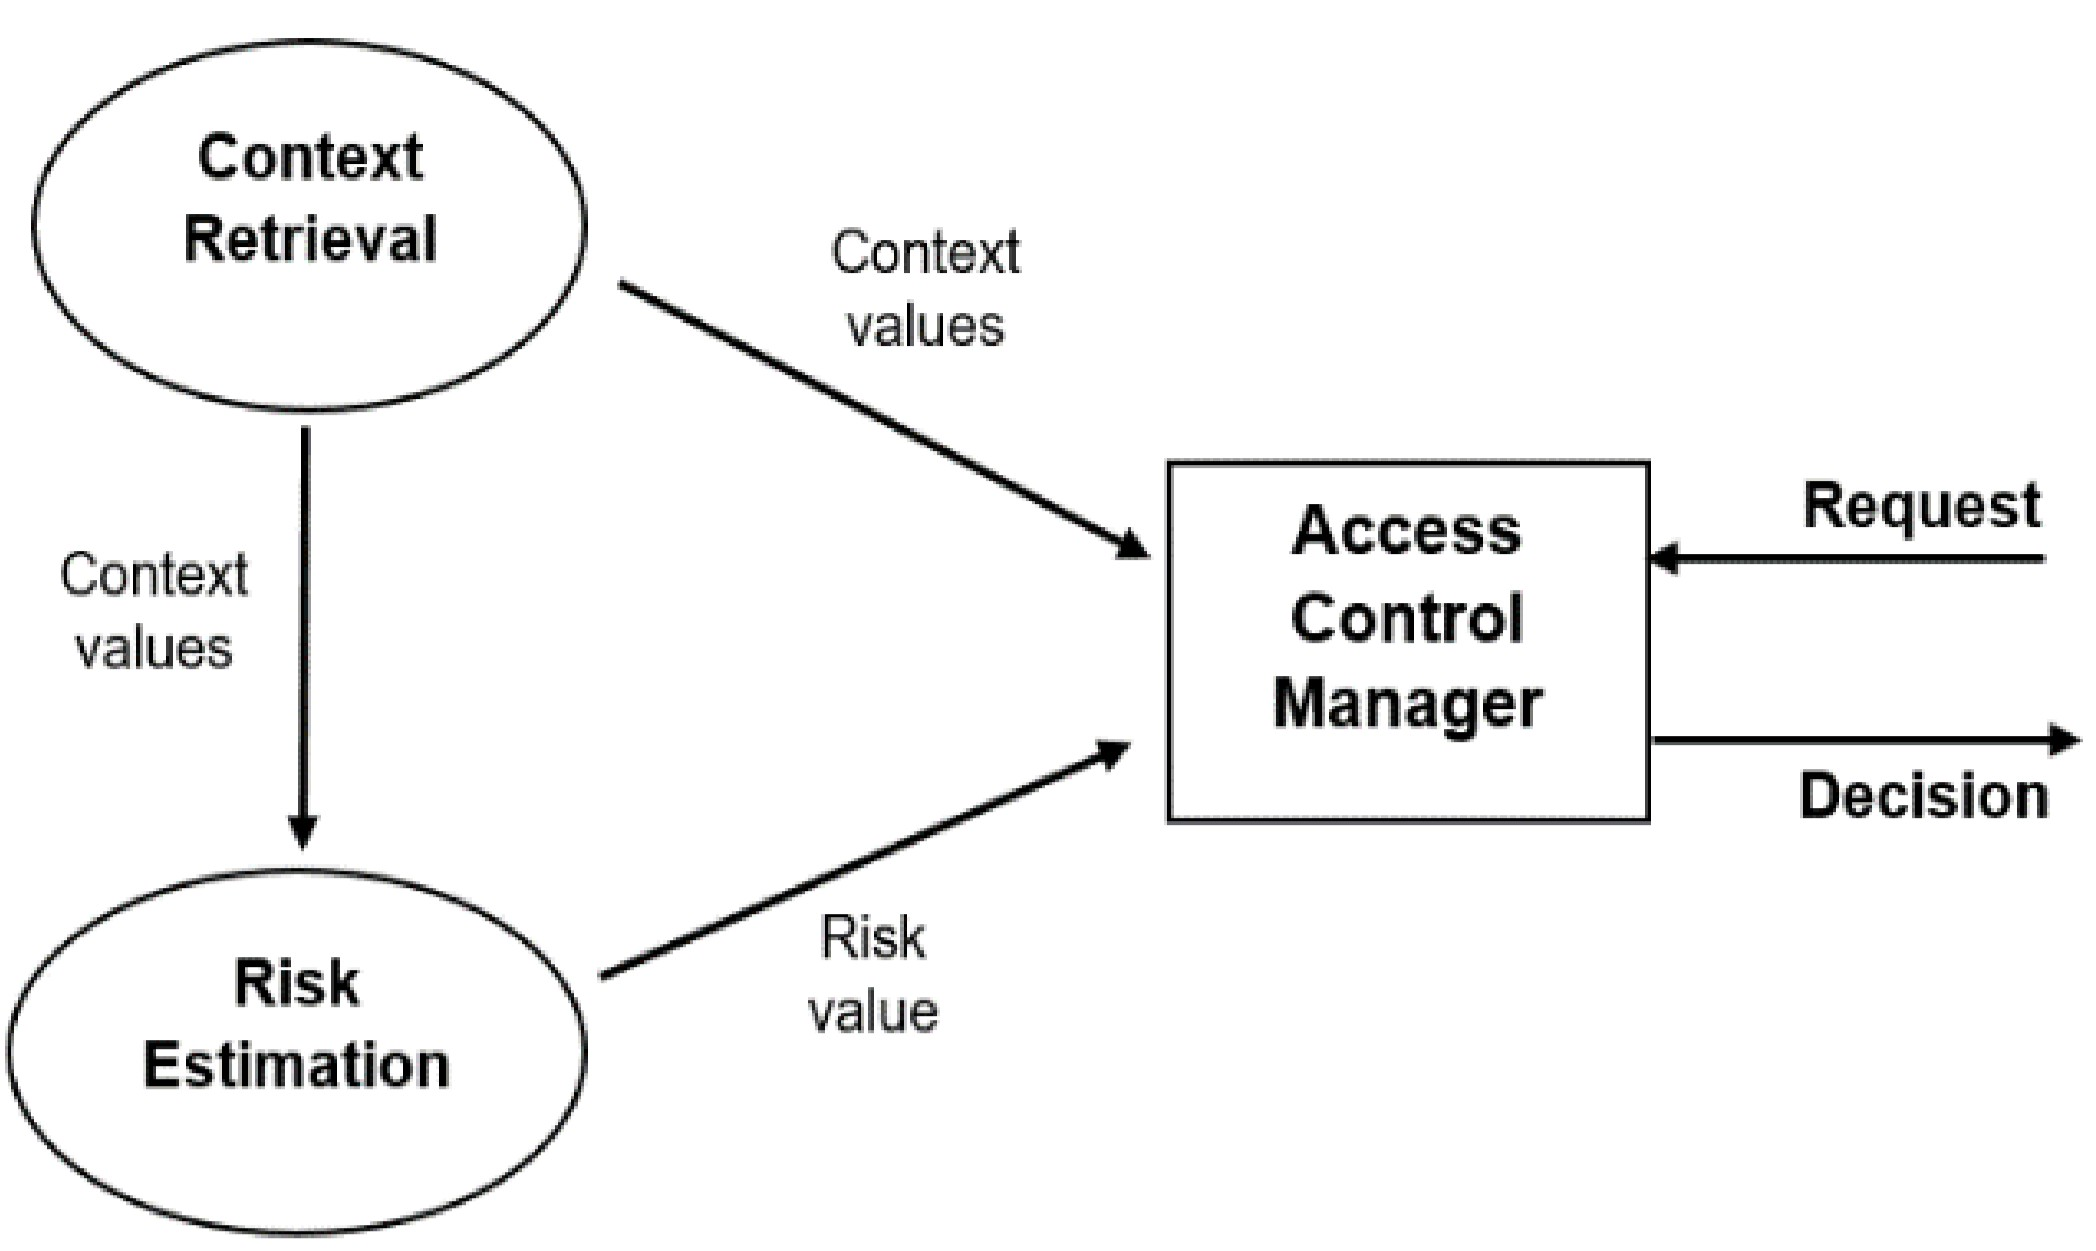
\includegraphics[width=.85\textwidth]{./figures/fig-rbac.jpg}
	\caption{基于风险的访问控制概述\cite{diep2007}}\label{fig:rbac}
\end{figure}

在这项工作中,我们通过引入新的适应性风险估计方法和博弈论方法,扩展了基于风险的访问控制基本模型。具体来说,风险估算过程与公式\ref{eq:naive_risk}中的模型有所不同;基于博弈论方法的组件是一个新的建议。提议的框架包括新的组成部分,将在第\ref{sec:framework}节中介绍。


\section{符号和模型}
\label{sec:notations}


在由服务提供商$\mathbf{S}$(即系统)持有的大规模用户$\mathbf{U}$(即主题)和隐私敏感资源(即对象$\mathbf{O}$)组成的系统中,所有用户都希望尽可能多地访问资源(甚至违反隐私权政策),并且希望尽可能多地访问所有资源。但是,用户必须履行自己的义务,并且不希望资源或服务提供商识别其恶意访问行为;资源(和/或服务提供商)希望尽早且尽可能多地识别恶意访问行为。因此,用户和服务提供商之间存在访问合作和隐私冲突。用户和资源都是自私的,因为他们希望获得最大的利益,他们将在每个访问回合中做出最佳选择以最大化自己的利益。对于特定用户$u \in \mathbf{U}$,其隐私侵犯行为与其他用户的隐私侵犯行为不同,因为他们的义务彼此不同。但是,组$g$中总是有一些用户,这些用户在系统中具有相同或相似的义务(例如,所有胸外科医生在医院的HIS中必须遵循类似的义务)。组$g$中的用户$u$的访问请求$q_u$想要访问某些资源$o_{u,q} \subset \mathbf{O}$,$o_{g} \subset \mathbf{O}$ 是组$g$的所有访问资源的资源集,如果$o_{u,q}$和$o_{g}$之间的距离小于用户/对象$s$的阈值$t_u$,则访问请求$q_u$不侵犯隐私;否则,$q_u$侵犯了隐私。这意味着,如果访问遵循具有类似义务的用户访问模式,则它会侵犯隐私。这种侵犯隐私的定义是合理的。因为同一组中的所有用户将以相似的方式执行其义务,因此遵循这些义务的所有访问都将以相似的方式执行。 一旦访问不遵循义务,则模式将有所不同,并且此访问侵犯了隐私。 在此,我们将$o_{u,q}$与$o_{g}$之间的距离$d(o_{u,q},o_{g})$定义为访问请求$q$的隐私风险$r_q$。
\begin{definition}[\textbf{隐私风险}]
	\label{def:privacy_risk}
	$o_{u,q}$和$o_{g}$之间的距离$d(o_{u,q},o_{g})$是隐私访问请求$q$的风险$r_q$ ,其中$o_{u,q}$ 表示用户$u \in g$的访问请求q的目标资源集,$o_{g}$表示用户组g的访问资源集。
\end{definition}

\begin{definition}[\textbf{侵犯隐私访问}]
	\label{def:privacy_violation_access}
	
	给定用户u的隐私阈值$t_u$和用户$u$的访问请求$q$。 如果 $r_q > t_u$,则$q$为\textit{隐私违法访问}; 否则,$q$是\textit{普通访问}。
\end{definition}



注意,可以根据不同用户的历史访问行为,将定义 \ref{def:privacy_violation_access}中的隐私阈值设置为不同的值。 特定用户的隐私阈值可以根据其历史访问行为(例如,使用贝叶斯方法或马尔可夫方法)在不同时期内变化。

在访问活动期间,在用户$\mathbf{U}$和对象$\mathbf{O}$之间有一个博弈(实际上是由服务提供者$\mathbf{S}$而不是对象来博弈)。 在博弈中,参与者集$\mathbf{A}=\{A_1,A_2,...,A_n\}$由用户$\mathbf{U}$和服务提供商$\mathbf{S}$组成,每个参与者 $A_i$都有一个策略集$St_{A_i}$,其中包含Ai的所有潜在动作。 对于一个访问过程中的所有参与者,都有一个回报函数$U_{A_1,A_2,...,A_n}$。 因此,$<\mathbf{A},\{St_{A_i}\},U_{A_1,A_2,...,A_n}>$是访问控制博弈模型。 在该模型中,策略和收益值与用户$\mathbf{U}$的访问隐私有关。

\section{基于风险自适应的访问控制}
\label{sec:framework}


在这一部分中,我们利用博弈论提出了一个基于风险适应性的访问控制模型的高层框架,并给出了该框架的详细工作流程。
\subsection{RaBAC框架}
\label{sec:hlframework}

\begin{figure}[htb]
	\centering
	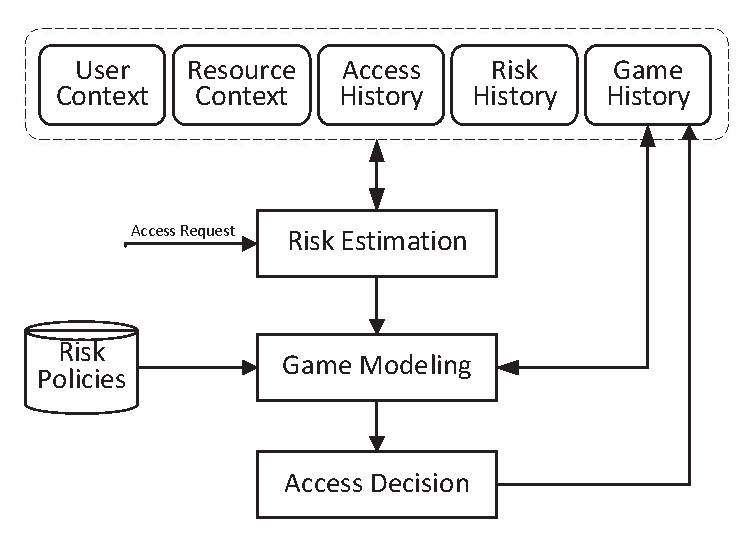
\includegraphics[width=.85\textwidth]{./figures/game-rbac-framework.eps}
	\caption{基于博弈论风险适应性的访问控制框架 (RaBAC)}\label{fig:game-rbac-framework}
\end{figure}



基于博弈论风险适应性的访问控制模型框架如图~\ref{fig:game-rbac-framework}所示。存储资源的系统记录所有用户$\mathbf{S}$的所有用户上下文,所有资源$\mathbf{O}$的资源上下文,用户$\mathbf{S}$的访问历史记录,每个访问请求$q$的风险历史记录,以及博弈参与者$\mathbf{A}$中的博弈历史记录。收到访问请求$q$后,系统会通过使用用户上下文,资源上下文,访问历史记录和风险历史记录来自适应地评估$q$的隐私风险$r_q$,并更新风险历史记录(风险估算模块) ;然后,系统尝试通过识别$q$是否是违反隐私的行为来识别请求访问$q$的用户$u$的访问策略$A_u$,系统会根据用户的访问策略执行最佳策略$A_u$以获取最大利益,并更新博弈历史记录(博弈建模模块);系统采取的最佳策略是接收到的访问请求$q$的访问决策(访问决策模块)。如第~\ref{sec:notations}节中所述,可以定期更新“风险策略”模块中每个用户的风险阈值。
在此框架中,风险估计和博弈建模是核心模块,风险评估模块旨在实现对访问控制的适应性隐私风险评估,博弈建模模块旨在实现针对访问控制的最佳策略选择。


\subsection{RaBAC的工作流程}


基于~\ref{sec:hlframework}的第~\ref{sec:framework}节中提出的框架,我们建议采用博弈论的风险适应性基本访问控制的显式工作流程。

在XACML的标准框架中,有四个组件,策略执行点(PEP),策略决策点(PDP),策略访问点(PAP)和策略信息点(PIP)。 策略执行点(PEP)收到用户的访问请求后,它将请求传递给策略决策点(PDP),然后PDP向策略访问点(PAP)和策略信息点(PIP)请求其他信息,然后进行 决定接受还是拒绝该请求。 另外,策略执行点(PEP)难以处理与请求者的交互,策略访问点(PAP)是静态的。 义务服务和策略信息点(PIP)都缺乏风险管理。


在我们提出的模型中,对PEP,PIP和PAP进行了改进,并添加了新的三个组件,即博弈建模,策略风险评估点(PREP),会话控制和风险缓解服务。 然后,一旦PDP接收到来自经过身份验证的用户的访问请求,并且在做出决定之前,它会请求与指定用户和历史记录相关的风险值,并构建一个博弈模型来做出决定。 此外,在由博弈建模组件执行决策后,一些反馈信息将提供给义务服务。 PREP可以实现对访问请求和用户的适应性隐私风险估计,博弈建模组件可以在用户(对象)和系统(对象)之间实现最佳访问策略选择。

\begin{figure}[htb]
	\centering
	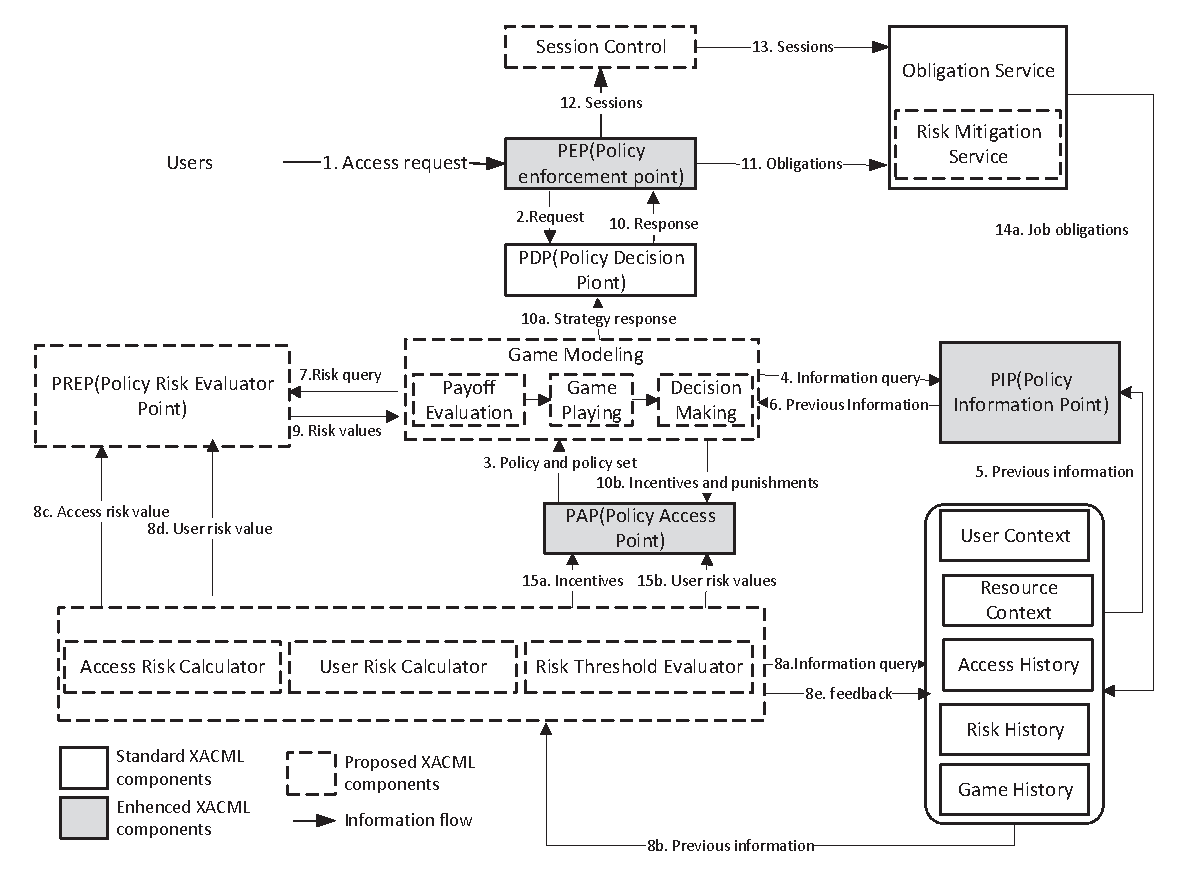
\includegraphics[width=1\textwidth]{./figures/game-rbac-workflow.eps}
	\caption{基于XACML的博弈理论RaBAC的处理流程}\label{fig:game-rbac-workflow}
\end{figure}


所提出的博弈论RaBAC的过程流程如图~\ref{fig:game-rbac-workflow}.显示了拟议的博弈理论RaBAC的处理流程。基于标准可扩展访问控制标记语言(XACML)提出了此框架。我们方法中的所有新组件均以虚线突出显示,所有增强的组件均以浅灰色突出显示。工作流基于标准XACML,所有访问请求均由经过身份验证的用户发送。从步骤1到6,组件传递请求并收集先前的信息以进行访问控制;在查询了风险值之后(步骤7),策略风险评估器点(PREP)估计访问的隐私风险值和用户风险值(步骤8)。注意,PREP由访问风险计算器,用户风险计算器和风险阈值评估器组成。每个请求都有一个风险值和用户风险值,并且会根据基础用户的过去行为(例如,用户上下文,资源上下文,访问历史记录和风险历史记录)评估这两个值。如果系统没有足够的历史记录,则PREP将根据建议评估两个值。与特定请求相关联的当前风险值返回到博弈建模(步骤9)。基于风险值,风险值和历史博弈行为,博弈建模为系统做出决策(例如,授予访问权限或拒绝访问权限)。将此决定转发给PEP,由其执行(步骤10)。无论是允许访问还是拒绝访问,PEP都会通知(步骤11)义务服务,该服务将决定是否需要风险缓解服务。在强制执行的延迟时间内,会话控制组件监视用户的行为,并管理访问会话(步骤12)。如果在此会话中访问行为的风险过高,则会话控制会通知义务服务组件并控制此会话中的请求(步骤13)。义务服务将决定是奖励还是惩罚用户,并更新用户的特征(步骤14)。 PAP定期更新激励对策和用户的用户风险值(步骤15)。

\section{私隐风险评估}
\label{sec:riskvalue}

风险评估是基于风险的访问控制的核心问题,设计一种适用于风险评估的方法很重要,因此可以实现基于风险适应性的访问控制模型。 在本节中,出于适应性隐私保护的目的,分别提出了针对访问请求和用户的适应性隐私风险估计方法。 这些方法是PREP组件的细节,如图所示~\ref{fig:game-rbac-workflow}

\subsection{访问请求的隐私风险}

除了我们在上一节中提出的框架之外,一个问题是如何评估来自用户的每个访问请求的隐私风险。 对于来自用户$u$的特定访问请求$q_u$,可以通过遵循定义~\ref{def:privacy_risk}来估算\emph{隐私风险} $r_{q_u}$



这是一个用户组$g$,其中$u \in g$,$g$中的所有用户都执行相似的义务,并且他们通过遵守义务来访问相似的资源。 假设在特定时期$t$(例如24小时或1周),$g$的用户总共访问了基础系统$n$次,并且访问请求为$Q^g_{pre}=(q^g_1,q^g_2,...,q^g_n)$,每个请求$q^u_i$旨在访问资源集$R^g_i$,其中$1 \leq i \leq n$。
现在,$q_u$是$u$的当前访问请求,而$R_u$是预期资源集。 因此,可以通过使用$R_{q_u}$的信息和$R^g_i$的平均信息之间的距离来估计\emph{privacy risk} $r_{q_u}$,如下

\begin{equation}\label{eq:privacy_risk_qu}
r_{q_u} = \dfrac{|Infor(R_{q_u})-\dfrac{\sum ^{n}_{i=1} Infor(R^g_i)}{n}|}{\dfrac{\sum ^{n}_{i=1} Infor(R^g_i)}{n}}, 
\end{equation}

其中$Infor(\cdot)$表示资源集$\cdot$的信息。 在一段时间内,组$g$中的所有用户访问资源都遵循一个分布。 可以通过每个访问请求中资源的访问频率来构造此分布。 因此,访问资源集$R^g = \bigcup _{i=1}^n R^g_i=\{x_1, x_2, \cdots, x_m\}$遵循分布

\begin{equation}\label{eq:distribution_Rg}
\left(
\begin{array}{c}
X \\ P(X)
\end{array}
\right)
=\left(
\begin{array}{cccccccccc}
x_1 &  x_2 & \cdots & x_m
\\ p(x_1) &  p(x_2) & \cdots & p(x_m)
\end{array}
\right),
\end{equation}

其中$p(x_j)=frequency(x_j)/\sum_{k=1}^m frequency(x_k)$,而$frequency(x_j)$表示$R^g_1, R^g_2, \cdots, R^g_n$中$x_j$的访问计数 。因此, $R^g_i =\{x_1^{R^g_i},x_2^{R^g_i},\cdots, x_t^{R^g_i}\} \subset R^g$,有

\begin{equation}\label{eq:information_Rgi}
Infor(R^g_i)=-\sum_{j=1}^t log(p(x_j^{R^g_i})).
\end{equation}


对于当前访问请求$q_u$的预期资源集$R_{q_u}$,可以将其分为两个子集: $R_{q_u}^* = R_{q_u}/R^g$ and $R_{q_u}^{**} = R_{q_u} \cap R^g = \{x_1^{R_{q_u}^{**}},x_2^{R_{q_u}^{**}},\cdots, x_r^{R_{q_u}^{**}}\}$,和

\begin{equation}\label{eq:information_Rqu}
\begin{split}
Infor(R_{q_u})&=Infor(R_{q_u}^{*})  +Infor(R_{q_u}^{**})
\\&=-\|R_{q_u}^*\|\cdot log(min(P(X)))-\sum_{j=1}^r log(p(x_j^{R_{q_u}^{**}})),
\end{split}
\end{equation}

其中$||R_{q_u}^*||$表示$R_{q_u}^*$的顺序。 在等式\ref{eq:information_Rqu}中,如果$R_{q_u}^* \neq \emptyset$,则$R_{q_u}^*$的任何元素都不属于$R^g$,并且我们使用 $R_g$代表它们。

在等式中\ref{eq:privacy_risk_qu},$r_{q_u} \geq 0$,并且$r_{q_u}$越大,$q_u$的隐私风险就越高。 我们可以在每个周期或每次访问中为用户$u$设置阈值$r_{q_u}^{th}$。 由定义\ref{def:privacy_violation_access},如果$r_{q_u} > r_{q_u}^{th}$,则$q_u$是违反隐私的访问;否则,$q_u$是普通访问,并且可以根据$u$的历史访问行为在每个周期或每次访问中更新$r_{q_u}^{th}$。

\subsection{用户风险计算}

在每个周期的开始,都有一个由服务提供商签署的用户${u}$的初始风险值${r_u ^ 0}$。 每次访问后,将根据基础访问来更新用户${u}$的风险值。 假设用户${u}$第${{i-1}}$次访问后的风险值为${r_u ^ {i-1}}$,并且${q_u}$是${u}$的当前访问请求,则该风险$ {u}$的值将更新为${r_u ^ {i}}$。 如果${q_u}$是违反隐私的访问,则${u}$的风险值将增加,反之则降低。 并且该值快速增加而缓慢减小。 这在我们的日常生活中自然而然,存在特定人的风险,如果他的表现不好,则风险会增加,而如果表现良好,则风险会降低。 即使他做了一些新的好事,他周围的人也会保持警惕,风险值也不会迅速下降。 如果他做了一些新的坏事,周围的人会更加警惕他,风险会迅速增加。 在这里,我们将用户的风险设置为

\begin{equation}\label{eq:userrisk}
r_u^{i}=\left\{ 
\begin{array}{cl}
r_u^{i-1}(1-\dfrac{\alpha}{xr_{max}}), & \text{if } q_u \text{ is a normal access;}\\
r_u^{i-1}(1+\dfrac{\beta}{r_{max}})), & \text{otherwise.}
\end{array}
\right.
\end{equation}

在等式\ref{eq:userrisk}中,$\alpha$和$\beta$是因子,$s$是连续正常访问的计数,$r_{max}$是最大的用户风险。

\section{博弈理论模型}
\label{sec:gamemodel}

\subsection{RaBAC的博弈模型}

博弈论是一种重要的数学工具,可用于与冲突和合作的参与者进行决策~\cite{owen2001}。
在访问控制系统中,服务提供商(系统)和用户(或多个用户)对不同的利益感兴趣,并且他们必须彼此合作以实现自己的利益。在这项工作中,我们假设服务提供商(系统)和用户是理性的,并且将基于风险适应性的访问控制建模为一种隐私保护的博弈模型,其中涉及参与者,参与者的策略和支付功能的参与者。在这个博弈中,有两个参与者,服务提供者$s$和用户$u$。服务提供商拥有对隐私敏感的资源(即对象),并希望授予正常访问权限并拒绝侵犯隐私的访问权限;用户是主体,谁希望为经济或其他利益而尽可能多地访问这些对象。用户$u$有两种策略,执行普通访问$N$和执行违反隐私的访问$V$;服务提供商有两种策略,分别授予访问权限$G$和拒绝访问权限$D$。~\ref{tab:payoff}显示了具有不同策略的参与者的支付功能。
\begin{table}[htb]
	\caption{服务提供商和用户之间的支付矩阵}\label{tab:payoff}
	\centering 
	\begin{tabular}{cccc}
		\toprule
		\multicolumn{2}{c}{\multirow{2}{*}{}} & \multicolumn{2}{c}{User} \\
		\cline{3-4}
		& & $N$ & $V$ \\	
		\hline
		\multirow{2}{*}{Service Provider} & $G$ &$U_s^{G,N}$, $U_u^{G,N}$ & $U_s^{G,V}$, $U_u^{G,V}$\\
		\cline{2-4}
		& $D$ & $U_s^{D,N}$, $U_u^{D,N}$ & $U_s^{D,V}$, $U_u^{D,V}$\\
		\toprule
	\end{tabular}
\end{table}


因此,基于风险适应性的访问控制的博弈模型可以由元组$<s,u,A_s,A_u,U_{s,u}>$定义,其中$s$是服务提供者,$u$是用户$A_s=\{G,D\}$是$s$的策略集,$A_u=\{N,V\}$是$u$的策略集,而$U_{s,u}=\{U_s^{G,N}, U_s^{G,V}, U_s^{D,N}, U_s^{D,V}, U_u^{G,N}, U_u^{G,V}, U_u^{D,N}, U_u^{D,V}\}$是具有不同策略的参与者的收益函数集。 该博弈是一个多阶段博弈,在每次迭代中,博弈者彼此了解并了解策略,同时,收益还取决于策略,历史访问和历史博弈策略。 因此,该博弈具有以下特征。
\begin{itemize}
	\item 两个博弈者的博弈:在每次访问迭代中,博弈者都是服务提供者和用户。
	\item 有限策略博弈:服务提供商和用户,分别具有两个可选策略。
	\item 非零和合作博弈:如果服务提供商和用户彼此合作,则均可获胜。 例如,如果用户执行常规访问并且服务提供商准予访问,则它们将共同受益。
	\item 静态博弈:在每次迭代之前,两个博弈者都不知道彼此的策略。
	\item 完美的信息博弈:博弈者知道他们在较早的访问迭代中选择了哪些策略。
	\item 不完整的信息博弈:在此博弈中,用户出于不同的兴趣爱好而具有不同的类型,并且服务提供商只是根据访问要求知道用户类型的分布。 在不同的访问迭代中,收益是不同的。
\end{itemize}

\subsection{博弈模型分析}

在表~\ref{tab:payoff}中,支付函数如下所示,并且我们分析了支付的组成部分。

\begin{itemize}
	\item $U_s^{G,N} >0$是授予正常访问权限时服务提供商的实用程序。该实用程序是服务提供商通过授予常规访问权限而获得的收益,并且该收益取决于基础访问权$q_u$和用户的风险值$r_u$。然后$U_s^{G,N}= Sbenefit_g^n\times (r_{max}-r_u)$​​,其中$Sbenefit_g^n$是服务提供商授予正常访问权限的基本好处,而$(r_{max}-r_u)$​​是因素。用户风险越低,服务提供商将获得更多的利益。
	\item $U_s^{G,V}<0$是授予隐私侵犯访问权限时服务提供商的实用程序。此实用程序是由于授予基本的隐私违规访问而导致的隐私丢失,并且受用户风险和访问风险的影响。然后$U_s^{G,V}= Sloss_g^v \times r_u \times r_{q_u}$。
	\item $U_s^{D,V} = 0$是拒绝隐私侵犯访问时服务提供商的实用程序。
	\item $U_u^{G,N}$是用户被授予正常访问权限时的实用程序。此实用程序是正常访问带来的收益,并受用户风险值影响,然后$U_u^{G,N}= Ubenefit_g^n \times(r_{max} - r_u)$。
	\item $U_u^{G,V} >0$是授予用户隐私权访问权限时的实用程序。该实用程序包括几个部分,正常利益和通过授予基本访问权而带来的额外利益,并受用户和访问权的当前风险的影响。然后$U_u^{G,V}= Ubenefit_g^n\times(r_{max} - r_u) + Uextra_g^v \times r_u\times r_{q_u}$
	\item $U_u^{D,N} =0$是拒绝用户正常访问时的实用程序。
	\item $U_u^{D,V}<0$是当用户的隐私违规访问被拒绝时的实用程序。该实用程序是服务提供商对用户的一种惩罚,并受到用户和访问风险的影响。然后$U_u^{D,V}= Upunish \times r_u \times r_{q_u}$。
\end{itemize}

在此多阶段博弈中,我们可以分离每个阶段之间的战略关系,并将每个子博弈视为一个独立博弈。假设此博弈中有$T$个阶段,并且$\sigma_1^*, \sigma_2^*, \cdots, \sigma_T^*$是独立阶段博弈的纳什均衡策略的有序序列,然后 存在子博弈的完美均衡,并且均衡路径由$\sigma_1^*, \sigma_2^*, \cdots, \sigma_T^*$生成。在每个阶段的博弈中,我们都会解决最佳策略。我们假设博弈中服务提供者的混合策略是$(p,1-p)$,其中服务提供者以概率$p$授予访问请求,并以概率$1-p$拒绝访问请求;并且用户的混合策略是$(q,1-q)$,其中{$ q $}是用户执行正常访问的概率,而$1-q$是执行隐私的概率用户违反访问权限。因此,用户的预期效用为
\begin{equation}
\begin{split}
U_u&= (1-q)(p\times U_u^{G,N}+ (1-p)\times U_u^{D,N})+ q(p\times U_u^{G,V}+(1-p)\times U_u^{D,V})\\
&=(1-q)\times p \times Ubenefit_g^n \times(r_{max} - r_u)+ q[p(Ubenefit_g^n\times(r_{max} - r_u) \\
&+ Uextra_g^v r_ur_{q_u})+(1-p)Upunishr_ur_{q_u}].
\end{split}
\end{equation}

通过求解微分方程$\frac{\partial U_n}{\partial q}=0$, we obtain $(p^*,1-p^*)$,我们得到$(p^*,1-p^*)$,其中
\begin{equation}
p^*=\dfrac{Upunish}{Upunish-Uextra_g^v}.
\end{equation}

因此,$(p^*,1-p^*)$是服务提供商混合策略的纳什均衡。在这种情况下,服务提供商希望惩罚并减少隐私侵犯访问。同样,我们可以为用户获得混合策略$(q^*,1-q^*)$的纳什均衡,其中
\begin{equation}
q^*=\dfrac{Sloss_g^v r_u r_{q_u}}{Sloss_g^v r_u  r_{q_u} +(Sloss_d^n -Sbenefit_g^n)(r_{max}-r_u)}.
\end{equation}

在这种情况下,服务提供商和用户都可以获得最大的收益,并且每个阶段的博弈都可以达到纳什均衡。因此,用户将要执行正常访问,而服务提供商将准许用户的正常访问请求。 因此,服务提供商通过限制隐私侵害访问来保留信息资源中涉及的隐私。

\section{比较与分析}
\label{sec:comparison}

尽管有文献\cite{ni2010risk,wang2011quantified,shaikh2012dynamic,santos2016,wang2019,zhang2015,zhen2015,zhang2018privacy,gao2018,liu2016,helil2017,hu2014,ding2019}报道了与风险或博弈论相关的不同访问控制模型,但我们的工作与 这些报告和收益比它们更大。 比较显示在图~\ref{tab:comparison}中。

\begin{table}[htb]
	
	\caption{所提出模型与已有工作的对比}\label{tab:comparison}
	\centering 
	\tiny
	\begin{tabular}{ccccc}
		\toprule
		Literature & Purpose of Access Control & Risk Estimation & Players of Game & Game Model \\
		\hline
		Ni et al\cite{ni2010risk} & Security protection &Static security risk&-&-\\ 
		Shaikh et al\cite{shaikh2012dynamic} & Security protection & Dynamic risk and trust &-&-\\
		dos Santos et al\cite{santos2016} &Cloud security protection & Multi-factor aggregation risk &-&-\\
		Ding et al\cite{ding2019} & Cloud  data security protection& Dynamic risk via entropy and Markov & - & -\\
		Wang and Jin\cite{wang2011quantified} & Privacy preserving of medical information & Static privacy risk &-&-\\
		Zhen et al\cite{zhen2015} & Privacy preserving of medical information& Dynamic risk via entropy & - & -\\
		Zhang et al\cite{zhang2018privacy} & Privacy preserving of medical information& Dynamic privacy risk via conditional probability  and Markov &-&-\\
		Liu et al\cite{liu2016} & Access security of multi-femtocell networks&-&	Multi players&	Stackelberg game\\
		Gao et al\cite{gao2018} & Cloud  data security protection& -&	Two players &Repeat game\\
		Zhang et al\cite{zhang2015} & Security protection& Trust & Two players & Non-zero-sum multi-stage game\\
		Wang et al\cite{wang2019} & Security protection& Dynamic trust & Two players & Non-zero-sum multi-stage game\\
		Hu et al\cite{hu2014} & Privacy preserving of social network&Static privacy risk&Multi players&	Multi-control game\\
		Helil et al\cite{helil2017} & General access control scenarios&Dynamic security risk&Two players&Non-zero-sum cooperative game\\
		This work & Data privacy preserving& Dynamic privacy risk via information and Markov & Two players & Non-zero-sum multi-stage game\\
		\bottomrule 
	\end{tabular}
\end{table}



在表~\ref{tab:comparison}中,几个工作~\cite{ni2010risk,shaikh2012dynamic,santos2016,ding2019,wang2011quantified,zhang2018privacy,zhen2015}设计了基于混合风险的非混合访问控制。但是,Niel等人\cite{ni2010risk}和Shaikh等人\cite{shaikh2012dynamic}的目标是分别通过估计静态安全风险和动态风险来保护系统的安全。 dos Santos等人\cite{santos2016}和Ding等人\cite{ding2019}提出了基于风险自适应的访问控制模型,以通过不同的动态风险估算方法维护云安全性。我们的模型是为了在开放和数据集中式系统中保护隐私而不是安全保护,它适用于本地和云系统。尽管一些作者\cite{wang2011quantified,zhen2015,zhang2018privacy}提出了用于保护隐私的基于风险的不同访问模型,但是这些模型仅适用于医疗保健系统,并且可以保留病历的隐私,这些工作改进了风险估计的方法。我们的模型不仅可以应用于医疗保健系统,还可以应用于其他方案(例如,分类信息系统,数据集中系统)。此外,我们的隐私风险值包括通过Shannon信息和Markov访问请求和用户,而不是通过熵\cite{zhen2015}和条件概率\cite{zhang2018privacy}的静态隐私风险\cite{wang2011quantified}。此外,所有这些工作都是非博弈论方法,我们的工作是基于风险适应性的访问控制的博弈论方法。在我们提出的访问控制模型中,所有参与者都是理性和自私的,他们在每次访问迭代中都做出了最佳选择。


还有一些基于博弈论的访问控制模型\cite{liu2016,gao2018,zhang2015,wang2019,hu2014,helil2017}。 但是只有Hu等人\cite{hu2014}和Helil等人\cite{helil2017}的工作是基于风险的访问控制模型,而Liu等人\cite{liu2016}和Gao等人\cite{gao2018}只是利用博弈论扩展了传统的访问控制,并应用于多毫微微小区网络和云数据访问 控制方面,Zhang等人\cite{zhang2015}和Wang等人\cite{wang2019}专注于通过信任而不是风险进行安全保护。 甚至Zhang等人和Wang等人的模型都是两人非零和多阶段博弈,与我们的模型相同,其应用场景和估计方法也有所不同,例如 我们的模型用于数据隐私保护,并基于一种可调整的隐私风险估计方法。 除此之外,这些工作\cite{liu2016,gao2018,zhang2015,wang2019}都不是基于风险的访问控制,而我们的模型是基于风险适应性的访问控制。

最相似的报告是\cite{hu2014}和\cite{helil2017},它们是基于风险和博弈论的访问控制模型。但是这些作品与我们的作品不同。 Hu等\cite{hu2014}提出了一种用于通过静态隐私风险估计在社交网络中保护隐私的多方控制博弈。
我们的工作不是针对社交网络,博弈模型与Hu等人\cite{hu2014}不同,\cite{hu2014}的作者根据用户关系设计了静态隐私风险,而我们模型中的隐私风险则根据用户的历史访问权限是动态的和自适应的行为。在\cite{helil2017}中,作者针对一般访问控制方案提出了基于风险信任的访问控制的两人非零和合作博弈分析。这项工作不是为了保护隐私,并且该模型基于历史访问通过用户的信任值估计了许可风险。虽然我们的工作是在开放和数据集中的情况下保护隐私,并根据访问请求和用户的直接估计隐私风险。此外,我们还为访问控制模型提出了一个基于XACML的框架和详细的工作流程。

\section{小结}\label{sec:conclusions}

在这项工作中,出于保护访问控制系统中隐私的目的,我们提出了一种基于风险适应性的访问控制模型,并将此访问控制建模为一个多阶段的两人博弈。 在该模型中,引入了一些新的组件,例如风险评估和博弈建模,并通过使用Shannon信息来估计访问风险和用户风险。 最后,我们为每次访问迭代获得了子博弈的纳什均衡,服务提供商和用户都希望在这种状态下表现良好,并且通过限制侵犯隐私的访问请求来保护隐私敏感的资源。 比较表明,此访问控制模型比以前的工作受益更多,并且实现了良好的隐私保护性能。